% THIS DOCUMENT IS NOT FOR JUFO SUBMISSION
\documentclass[12pt,a4paper]{article}
\usepackage{amsmath,amssymb,amsthm}
\usepackage{graphicx}
\usepackage[margin=1in]{geometry}
\usepackage{enumitem}
\usepackage{hyperref}
\usepackage{url}
\usepackage{tikz}
\usepackage{tikz-cd}
\usepackage{tikz-3dplot}
\usetikzlibrary{angles,quotes,arrows.meta,calc,babel,3d,positioning}
\usepackage{lipsum}
\usepackage{listings}
\usepackage{fancyhdr}
\usepackage{xcolor} % Added for colors
\usepackage{titlesec} % Added for title formatting

% Define colors
\definecolor{titlecolor}{RGB}{0, 51, 102}

% Consistent theorem/proof environments
\newtheorem{theorem}{Theorem}
\newtheorem{lemma}[theorem]{Lemma}
\newtheorem{corollary}[theorem]{Corollary}
\theoremstyle{definition}
\newtheorem{definition}[theorem]{Definition}
\newtheorem{problem}{Problem}

% Set up headers
\pagestyle{fancy}
\fancyhf{} % Clear all header and footer fields
\fancyhead[L]{Victor Gurbani}
\fancyhead[R]{JuFo 2026}
\fancyfoot[C]{\thepage} % Page number in center of footer

% Define a separate first page style with no numbers
\fancypagestyle{firstpage}{
    \fancyhf{} % Clear all header and footer fields
    \renewcommand{\headrulewidth}{0pt} % Remove header rule
    \renewcommand{\footrulewidth}{0pt} % Remove footer rule
}

% Create a custom title command
\renewcommand{\maketitle}{
    \begin{titlepage}
        \centering
        \vspace*{1cm}
        {\color{titlecolor}\rule{\linewidth}{1pt}}
        \vspace{1.5cm}
        
        {\fontsize{28}{34}\selectfont\color{titlecolor}\textbf{Empirische Musikalische Kartographie} \par Die Analysierung der Landschaft harmonischer und melodischer Stile\par}
        
        \vspace{1.5cm}
        {\color{titlecolor}\rule{\linewidth}{1pt}}
        \vspace{2cm}
        
        {\Large\textbf{Victor Gurbani}\par}
        \vspace{0.5cm}
        {\large\today\par}
        
        \vfill
        % Optional: Add a simple decorative element
        % \begin{tikzpicture}[remember picture, overlay]
        %     \draw[color=titlecolor, line width=0.5pt] 
        %         ($(current page.center) + (-3,0)$) -- ($(current page.center) + (3,0)$);
        % \end{tikzpicture}
    \end{titlepage}
}

\begin{document}

\maketitle
\setcounter{page}{1}
\pagenumbering{arabic}
\newpage

\section{Abstract}
I assembled a license-safe corpus of 144 solo-piano scores (36 each by Bach, Mozart, Chopin, and Debussy) from the 254{,}077-score PDMX archive and built an end-to-end toolkit that quantifies harmonic, melodic, and rhythmic practice across the four composers. The pipeline extracts 36 interpretable features with \texttt{music21}, evaluates stylistic separation via ANOVA/Tukey tests, and publishes interactive embeddings plus score-level overlays in MuseScore. Early results show 29 of the metrics remain statistically significant after false-discovery control: chromatic density, dissonance rates, and rhythmic entropy clearly distinguish Chopin and Debussy from the classical pair, while range- and cadence-driven measures keep Bach and Mozart clustered. Principal-component embeddings reinforce this narrative, placing Chopin between classical clarity and impressionist colour and isolating Debussy in a distinct third region. All data, plots, and scripts are packaged for reproducible exploration of stylistic evolution.

\section{Two-Page Summary of Findings}

\subsection{Balanced Corpus and Parsing Pipeline}
Starting with 254{,}077 PDMX entries, I filtered by licensing, originality, instrumentation metadata, and a composer-normalisation scheme to isolate a strictly solo-piano subset. The final cohort contains 36 works per target composer (144 total), averaging 148.22 measures and 2.10 parts per piece and spanning 71{,}585 quarter-note durations (13.26 listening hours at 90~BPM). JSON metadata caching, arrangement detection, and instrumentation cross-checks ensure the remaining scores are genuine solo piano pieces rather than reductions or ensemble arrangements. A companion parsing script wraps disparate \texttt{music21} outputs (Score, Part, Opus) into a consistent \texttt{stream.Score} object, extracting measures, parts, and durations to produce reusable summaries under \texttt{data/parsed/}. This structural baseline prevents redundant MusicXML reads during later stages and enables quick sanity checks of corpus balance.


\subsection{Feature Engineering Across Three Pillars}
I engineered 36 descriptors: 16 harmonic, 11 melodic, and 9 rhythmic metrics. Harmonic analysis chordifies each score, computes chord-quality percentages, harmonic density, dissonance classifications (passing tones, appoggiaturas, other), and Roman numeral trends. Melodic features cover ambitus, interval statistics, leap ratios, pitch-class entropy, and soprano/bass interaction metrics (contrary, parallel, oblique motion). Rhythmic descriptors quantify duration spread, syncopation, downbeat emphasis, sliding-window entropy, micro-density of fast notes, and cross-hand subdivision mismatches. Each extractor offers CLI flags for limits, cached reuse, and optional boxplot generation, creating CSV outputs under \texttt{data/features/} and supporting documentation such as \texttt{Harmonic\_Features.md} and \texttt{Melodic\_Features.md}.

\subsection{Statistical Separation of Styles}
Running one-way ANOVA followed by Tukey HSD comparisons across the combined feature set surfaced strong stylistic separation across harmonic, melodic, and rhythmic domains. After a conservative Bonferroni correction, 14 features remain significant; with Benjamini--Hochberg false-discovery control, 29 robust metrics remain significant. Registral span (\emph{pitch\_range\_semitones}) and dissonance usage (\emph{dissonance\_ratio}) clearly separate Romantic and Impressionist writing from earlier styles (e.g., \emph{pitch\_range\_semitones}: $F=42.18$, $p<1.8\times10^{-19}$; \emph{dissonance\_ratio}: $F=30.65$, $p<2.7\times10^{-15}$). Rhythmic metrics such as \emph{std\_note\_duration} ($p\approx1.5\times10^{-10}$) and \emph{rhythmic\_pattern\_entropy} ($p\approx5.0\times10^{-10}$) differentiate Chopin and Debussy from Bach and Mozart, while \emph{syncopation\_ratio} remains a defining trait for Debussy. Figure~\ref{fig:anova} summarises the strongest omnibus tests, while Figure~\ref{fig:pair-heatmap} maps how often each composer pair diverges after excluding raw count features (e.g., Debussy--Mozart differs on 16 features, while Bach--Mozart differs on 10).

\begin{figure}[h]
    \centering
    \includegraphics[width=0.85\textwidth]{figures/significance/top_anova_bar.png}
    \caption{Top ANOVA hits across harmonic, melodic, and rhythmic feature families.}
    \label{fig:anova}
\end{figure}

\begin{figure}[h]
    \centering
    \includegraphics[width=0.85\textwidth]{figures/significance/tukey_pair_heatmap.png}
    \caption{Count of statistically significant features per composer pairing (Tukey HSD).}
    \label{fig:pair-heatmap}
\end{figure}


\newpage

\subsection{Interpreting the Embedding Landscape}
Principal-component embeddings clarify how stylistic traits blend. After standardising the feature matrix and excluding raw count columns, PCA explains 48.2\% of the variance in the first three components. Composer centroids at (Mozart~\textminus2.31, 0.83, \textminus0.45), (Bach~\textminus0.37, \textminus1.16, \textminus0.63), (Chopin~0.60, 0.04, 0.44), and (Debussy~2.08, 0.29, 0.64) reflect the axes' musical meaning: PC1 tracks chromatic density, leap ratio, and dissonance; PC2 contrasts long, downbeat-emphasised phrases with dense note streams; PC3 rewards oblique motion, cross-rhythms, and registral spread. Chopin bridges classical clarity and impressionist colour by sharing cadential discipline with Bach/Mozart (PC2) while adopting chromatic and rhythmic innovations that align him with Debussy (PC1/PC3). Debussy extends these traits, occupying a distinct ``third slot'' beyond Chopin. Interactive HTML views provide both point clouds and Gaussian ``composer clouds'' for browser-based exploration, augmented with directional lighting to enhance depth perception.

\subsection{Model Validation: The ``Ravel Test''}
To test whether the feature space is predictive beyond the training corpus, I projected an unseen external score: \textbf{Maurice Ravel's \textit{String Quartet in F Major}}. Using the same projection tooling (\texttt{highlight\_pca\_piece.py}) and a dark diamond marker for visibility, the model places Ravel in the expected post-impressionist direction: notably, \emph{further along the primary component axis than Debussy}. This supports the interpretation that the engineered features are not only descriptive of historical styles, but can generalise to later stylistic evolution.

\begin{figure}[htbp]
    \centering
    \IfFileExists{ravelhighlight_cropped.png}{%
        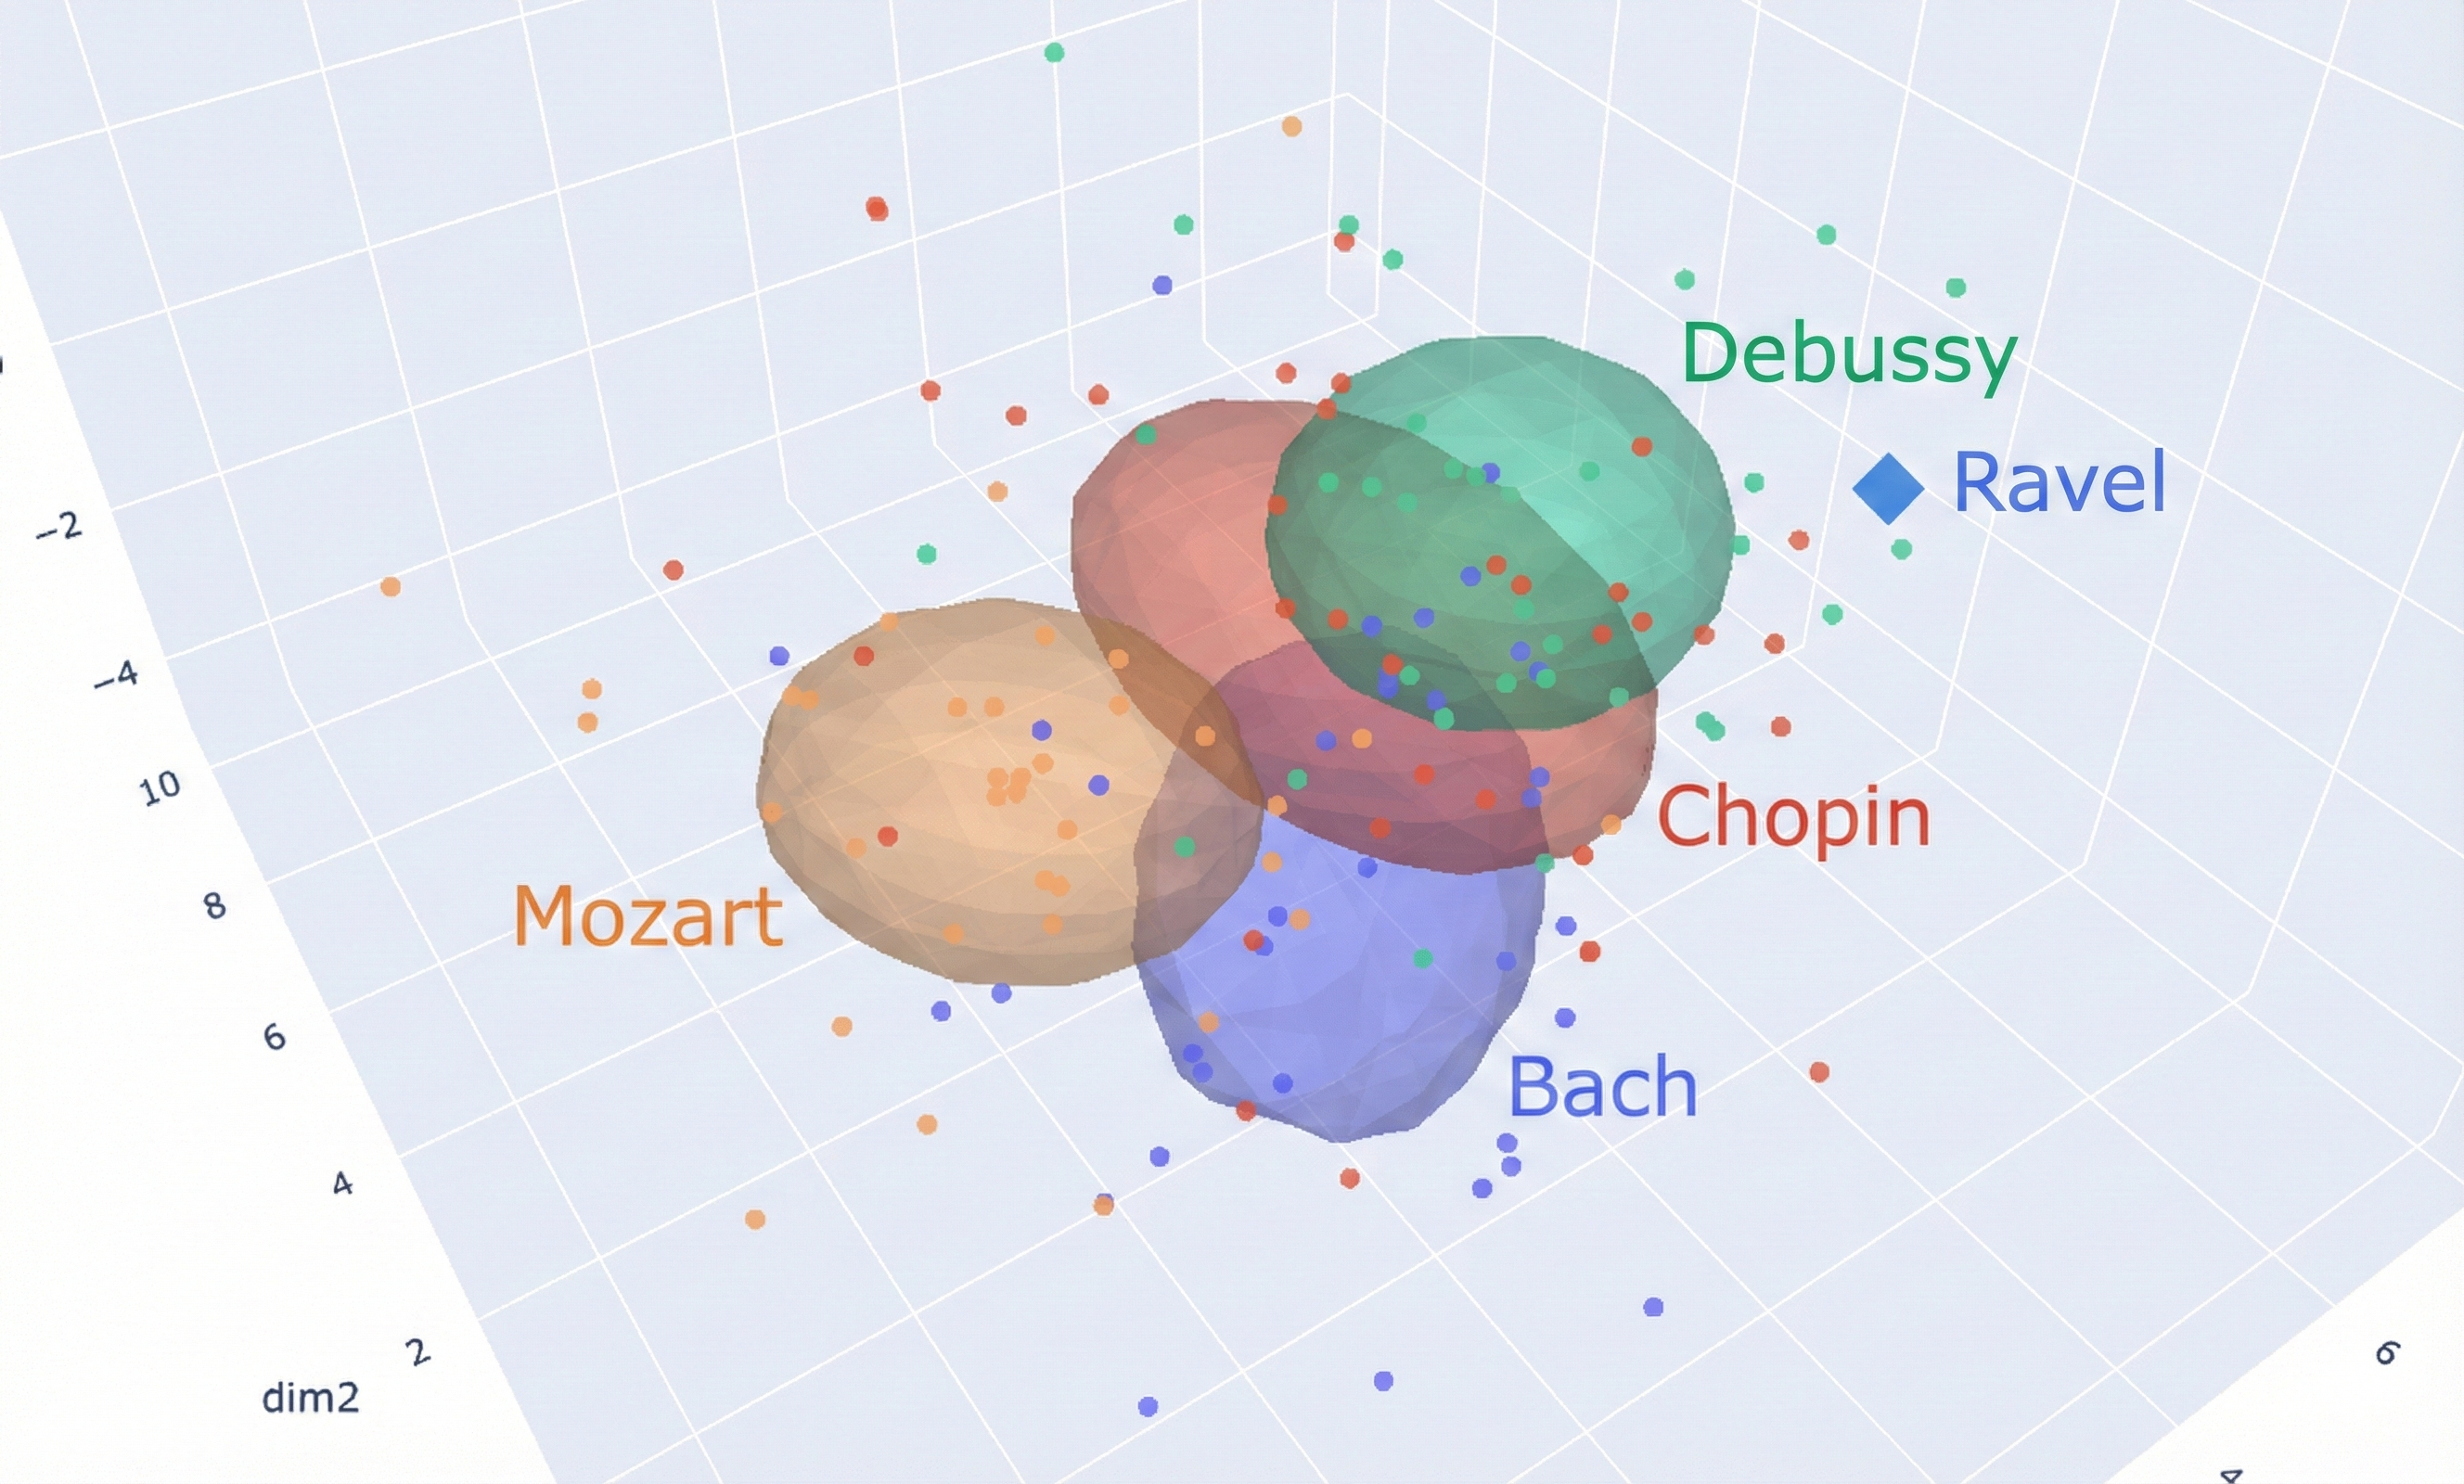
\includegraphics[width=0.85\textwidth]{ravelhighlight_cropped.png}
    }{%
        \fbox{\parbox{0.85\textwidth}{\centering (Missing figure file: ravelhighlight\_cropped.png)}}
    }
    \caption{External validation via PCA projection: the diamond marker denotes Ravel's \textit{String Quartet in F} projected into the learned stylistic space.}
    \label{fig:ravel-test}
\end{figure}

\begin{figure}[htbp]
    \centering 
    \includegraphics[width=0.85\textwidth]{figures/embeddings/composer_clouds_3d.png}
    \caption{3D PCA embedding showing composer clouds and stylistic separation across the first three principal components.}
    \label{fig:composer-clouds}
\end{figure}

\newpage

\subsection{Score-Level Evidence via Annotation}
To connect statistical findings to notation, the annotation pipeline enriches MusicXML files with coloured noteheads, lyric labels, chord symbols, and text expressions. Passing tones (orange), appoggiaturas (violet), other dissonances (red), and chromatic harmonies (turquoise) are flagged directly in the score. Chord symbols mirror Roman numeral analyses, and fallbacks ensure MuseScore displays readable figures even when automatic chord spelling fails. Batch scripts regenerate flagship works per composer and optionally invoke MuseScore's CLI to export PDF/PNG renditions, facilitating peer review without specialised software.

\subsection{Implications and Reuse}
Taken together, the curated dataset, multi-faceted feature suite, statistical evidence, and visual tooling deliver a reproducible laboratory for studying stylistic evolution from Baroque counterpoint to Impressionist colour. Analysts can reuse the CLI suite to test new hypotheses, integrate additional composers, or layer machine-learning models atop the harmonically balanced feature space. The documentation in and supporting markdown files captures both methodology and interpretive narratives, making the project portable for future musicology research.



\end{document}